% Options for packages loaded elsewhere
\PassOptionsToPackage{unicode}{hyperref}
\PassOptionsToPackage{hyphens}{url}
%
\documentclass[
]{article}
\usepackage{amsmath,amssymb}
\usepackage{iftex}
\ifPDFTeX
  \usepackage[T1]{fontenc}
  \usepackage[utf8]{inputenc}
  \usepackage{textcomp} % provide euro and other symbols
\else % if luatex or xetex
  \usepackage{unicode-math} % this also loads fontspec
  \defaultfontfeatures{Scale=MatchLowercase}
  \defaultfontfeatures[\rmfamily]{Ligatures=TeX,Scale=1}
\fi
\usepackage{lmodern}
\ifPDFTeX\else
  % xetex/luatex font selection
\fi
% Use upquote if available, for straight quotes in verbatim environments
\IfFileExists{upquote.sty}{\usepackage{upquote}}{}
\IfFileExists{microtype.sty}{% use microtype if available
  \usepackage[]{microtype}
  \UseMicrotypeSet[protrusion]{basicmath} % disable protrusion for tt fonts
}{}
\makeatletter
\@ifundefined{KOMAClassName}{% if non-KOMA class
  \IfFileExists{parskip.sty}{%
    \usepackage{parskip}
  }{% else
    \setlength{\parindent}{0pt}
    \setlength{\parskip}{6pt plus 2pt minus 1pt}}
}{% if KOMA class
  \KOMAoptions{parskip=half}}
\makeatother
\usepackage{xcolor}
\usepackage[margin=1in]{geometry}
\usepackage{color}
\usepackage{fancyvrb}
\newcommand{\VerbBar}{|}
\newcommand{\VERB}{\Verb[commandchars=\\\{\}]}
\DefineVerbatimEnvironment{Highlighting}{Verbatim}{commandchars=\\\{\}}
% Add ',fontsize=\small' for more characters per line
\usepackage{framed}
\definecolor{shadecolor}{RGB}{248,248,248}
\newenvironment{Shaded}{\begin{snugshade}}{\end{snugshade}}
\newcommand{\AlertTok}[1]{\textcolor[rgb]{0.94,0.16,0.16}{#1}}
\newcommand{\AnnotationTok}[1]{\textcolor[rgb]{0.56,0.35,0.01}{\textbf{\textit{#1}}}}
\newcommand{\AttributeTok}[1]{\textcolor[rgb]{0.13,0.29,0.53}{#1}}
\newcommand{\BaseNTok}[1]{\textcolor[rgb]{0.00,0.00,0.81}{#1}}
\newcommand{\BuiltInTok}[1]{#1}
\newcommand{\CharTok}[1]{\textcolor[rgb]{0.31,0.60,0.02}{#1}}
\newcommand{\CommentTok}[1]{\textcolor[rgb]{0.56,0.35,0.01}{\textit{#1}}}
\newcommand{\CommentVarTok}[1]{\textcolor[rgb]{0.56,0.35,0.01}{\textbf{\textit{#1}}}}
\newcommand{\ConstantTok}[1]{\textcolor[rgb]{0.56,0.35,0.01}{#1}}
\newcommand{\ControlFlowTok}[1]{\textcolor[rgb]{0.13,0.29,0.53}{\textbf{#1}}}
\newcommand{\DataTypeTok}[1]{\textcolor[rgb]{0.13,0.29,0.53}{#1}}
\newcommand{\DecValTok}[1]{\textcolor[rgb]{0.00,0.00,0.81}{#1}}
\newcommand{\DocumentationTok}[1]{\textcolor[rgb]{0.56,0.35,0.01}{\textbf{\textit{#1}}}}
\newcommand{\ErrorTok}[1]{\textcolor[rgb]{0.64,0.00,0.00}{\textbf{#1}}}
\newcommand{\ExtensionTok}[1]{#1}
\newcommand{\FloatTok}[1]{\textcolor[rgb]{0.00,0.00,0.81}{#1}}
\newcommand{\FunctionTok}[1]{\textcolor[rgb]{0.13,0.29,0.53}{\textbf{#1}}}
\newcommand{\ImportTok}[1]{#1}
\newcommand{\InformationTok}[1]{\textcolor[rgb]{0.56,0.35,0.01}{\textbf{\textit{#1}}}}
\newcommand{\KeywordTok}[1]{\textcolor[rgb]{0.13,0.29,0.53}{\textbf{#1}}}
\newcommand{\NormalTok}[1]{#1}
\newcommand{\OperatorTok}[1]{\textcolor[rgb]{0.81,0.36,0.00}{\textbf{#1}}}
\newcommand{\OtherTok}[1]{\textcolor[rgb]{0.56,0.35,0.01}{#1}}
\newcommand{\PreprocessorTok}[1]{\textcolor[rgb]{0.56,0.35,0.01}{\textit{#1}}}
\newcommand{\RegionMarkerTok}[1]{#1}
\newcommand{\SpecialCharTok}[1]{\textcolor[rgb]{0.81,0.36,0.00}{\textbf{#1}}}
\newcommand{\SpecialStringTok}[1]{\textcolor[rgb]{0.31,0.60,0.02}{#1}}
\newcommand{\StringTok}[1]{\textcolor[rgb]{0.31,0.60,0.02}{#1}}
\newcommand{\VariableTok}[1]{\textcolor[rgb]{0.00,0.00,0.00}{#1}}
\newcommand{\VerbatimStringTok}[1]{\textcolor[rgb]{0.31,0.60,0.02}{#1}}
\newcommand{\WarningTok}[1]{\textcolor[rgb]{0.56,0.35,0.01}{\textbf{\textit{#1}}}}
\usepackage{graphicx}
\makeatletter
\def\maxwidth{\ifdim\Gin@nat@width>\linewidth\linewidth\else\Gin@nat@width\fi}
\def\maxheight{\ifdim\Gin@nat@height>\textheight\textheight\else\Gin@nat@height\fi}
\makeatother
% Scale images if necessary, so that they will not overflow the page
% margins by default, and it is still possible to overwrite the defaults
% using explicit options in \includegraphics[width, height, ...]{}
\setkeys{Gin}{width=\maxwidth,height=\maxheight,keepaspectratio}
% Set default figure placement to htbp
\makeatletter
\def\fps@figure{htbp}
\makeatother
\setlength{\emergencystretch}{3em} % prevent overfull lines
\providecommand{\tightlist}{%
  \setlength{\itemsep}{0pt}\setlength{\parskip}{0pt}}
\setcounter{secnumdepth}{-\maxdimen} % remove section numbering
\usepackage{graphicx}
\ifLuaTeX
  \usepackage{selnolig}  % disable illegal ligatures
\fi
\IfFileExists{bookmark.sty}{\usepackage{bookmark}}{\usepackage{hyperref}}
\IfFileExists{xurl.sty}{\usepackage{xurl}}{} % add URL line breaks if available
\urlstyle{same}
\hypersetup{
  pdftitle={Honours Multivariate Continuous Assessment 1},
  pdfauthor={Molemo Mafora , Tashmira Subramoney , Tinotenda Mutsemi},
  hidelinks,
  pdfcreator={LaTeX via pandoc}}

\title{Honours Multivariate Continuous Assessment 1}
\author{Molemo Mafora , Tashmira Subramoney , Tinotenda Mutsemi}
\date{2024-02-18}

\begin{document}
\maketitle

\begin{center}\rule{0.5\linewidth}{0.5pt}\end{center}

\section{Question 1}
\subsection{Sample Mean Vectors}

The mean vector is defined as: \[
\bar{x}_{j} = \frac{1}{n}\sum_{j}x_{ij} 
\] Therefore the mean vector for each of the 5 time periods are:

\begin{table}[!h]
\begin{center}
\caption{Sample mean vectors for each of the five time periods}
\vspace{0.5cm}
\begin{tabular}{|c|c|c|c|c|}
\hline
\textbf{TimePeriod} & \textbf{MaxBreath} & \textbf{BasHeight} & \textbf{BasLength} & \textbf{NasHeight} \\
\hline
\textbf{1} & 131.367    & 133.600 & 99.167 & 50.533 \\
\textbf{2} & 132.367    & 132.700 & 99.067  & 50.233 \\
\textbf{3} & 134.467    & 133.800 & 96.033 & 50.567 \\
\textbf{4} & 135.500    & 132.300 & 94.533  & 51.967 \\  
\textbf{5} & 136.167    & 130.333 & 93.500 & 51.367 \\  
\hline
\end{tabular}
\end{center}
\end{table}

\newpage
\section{Question 2}
\subsection{Heat map of the correlation matrix}

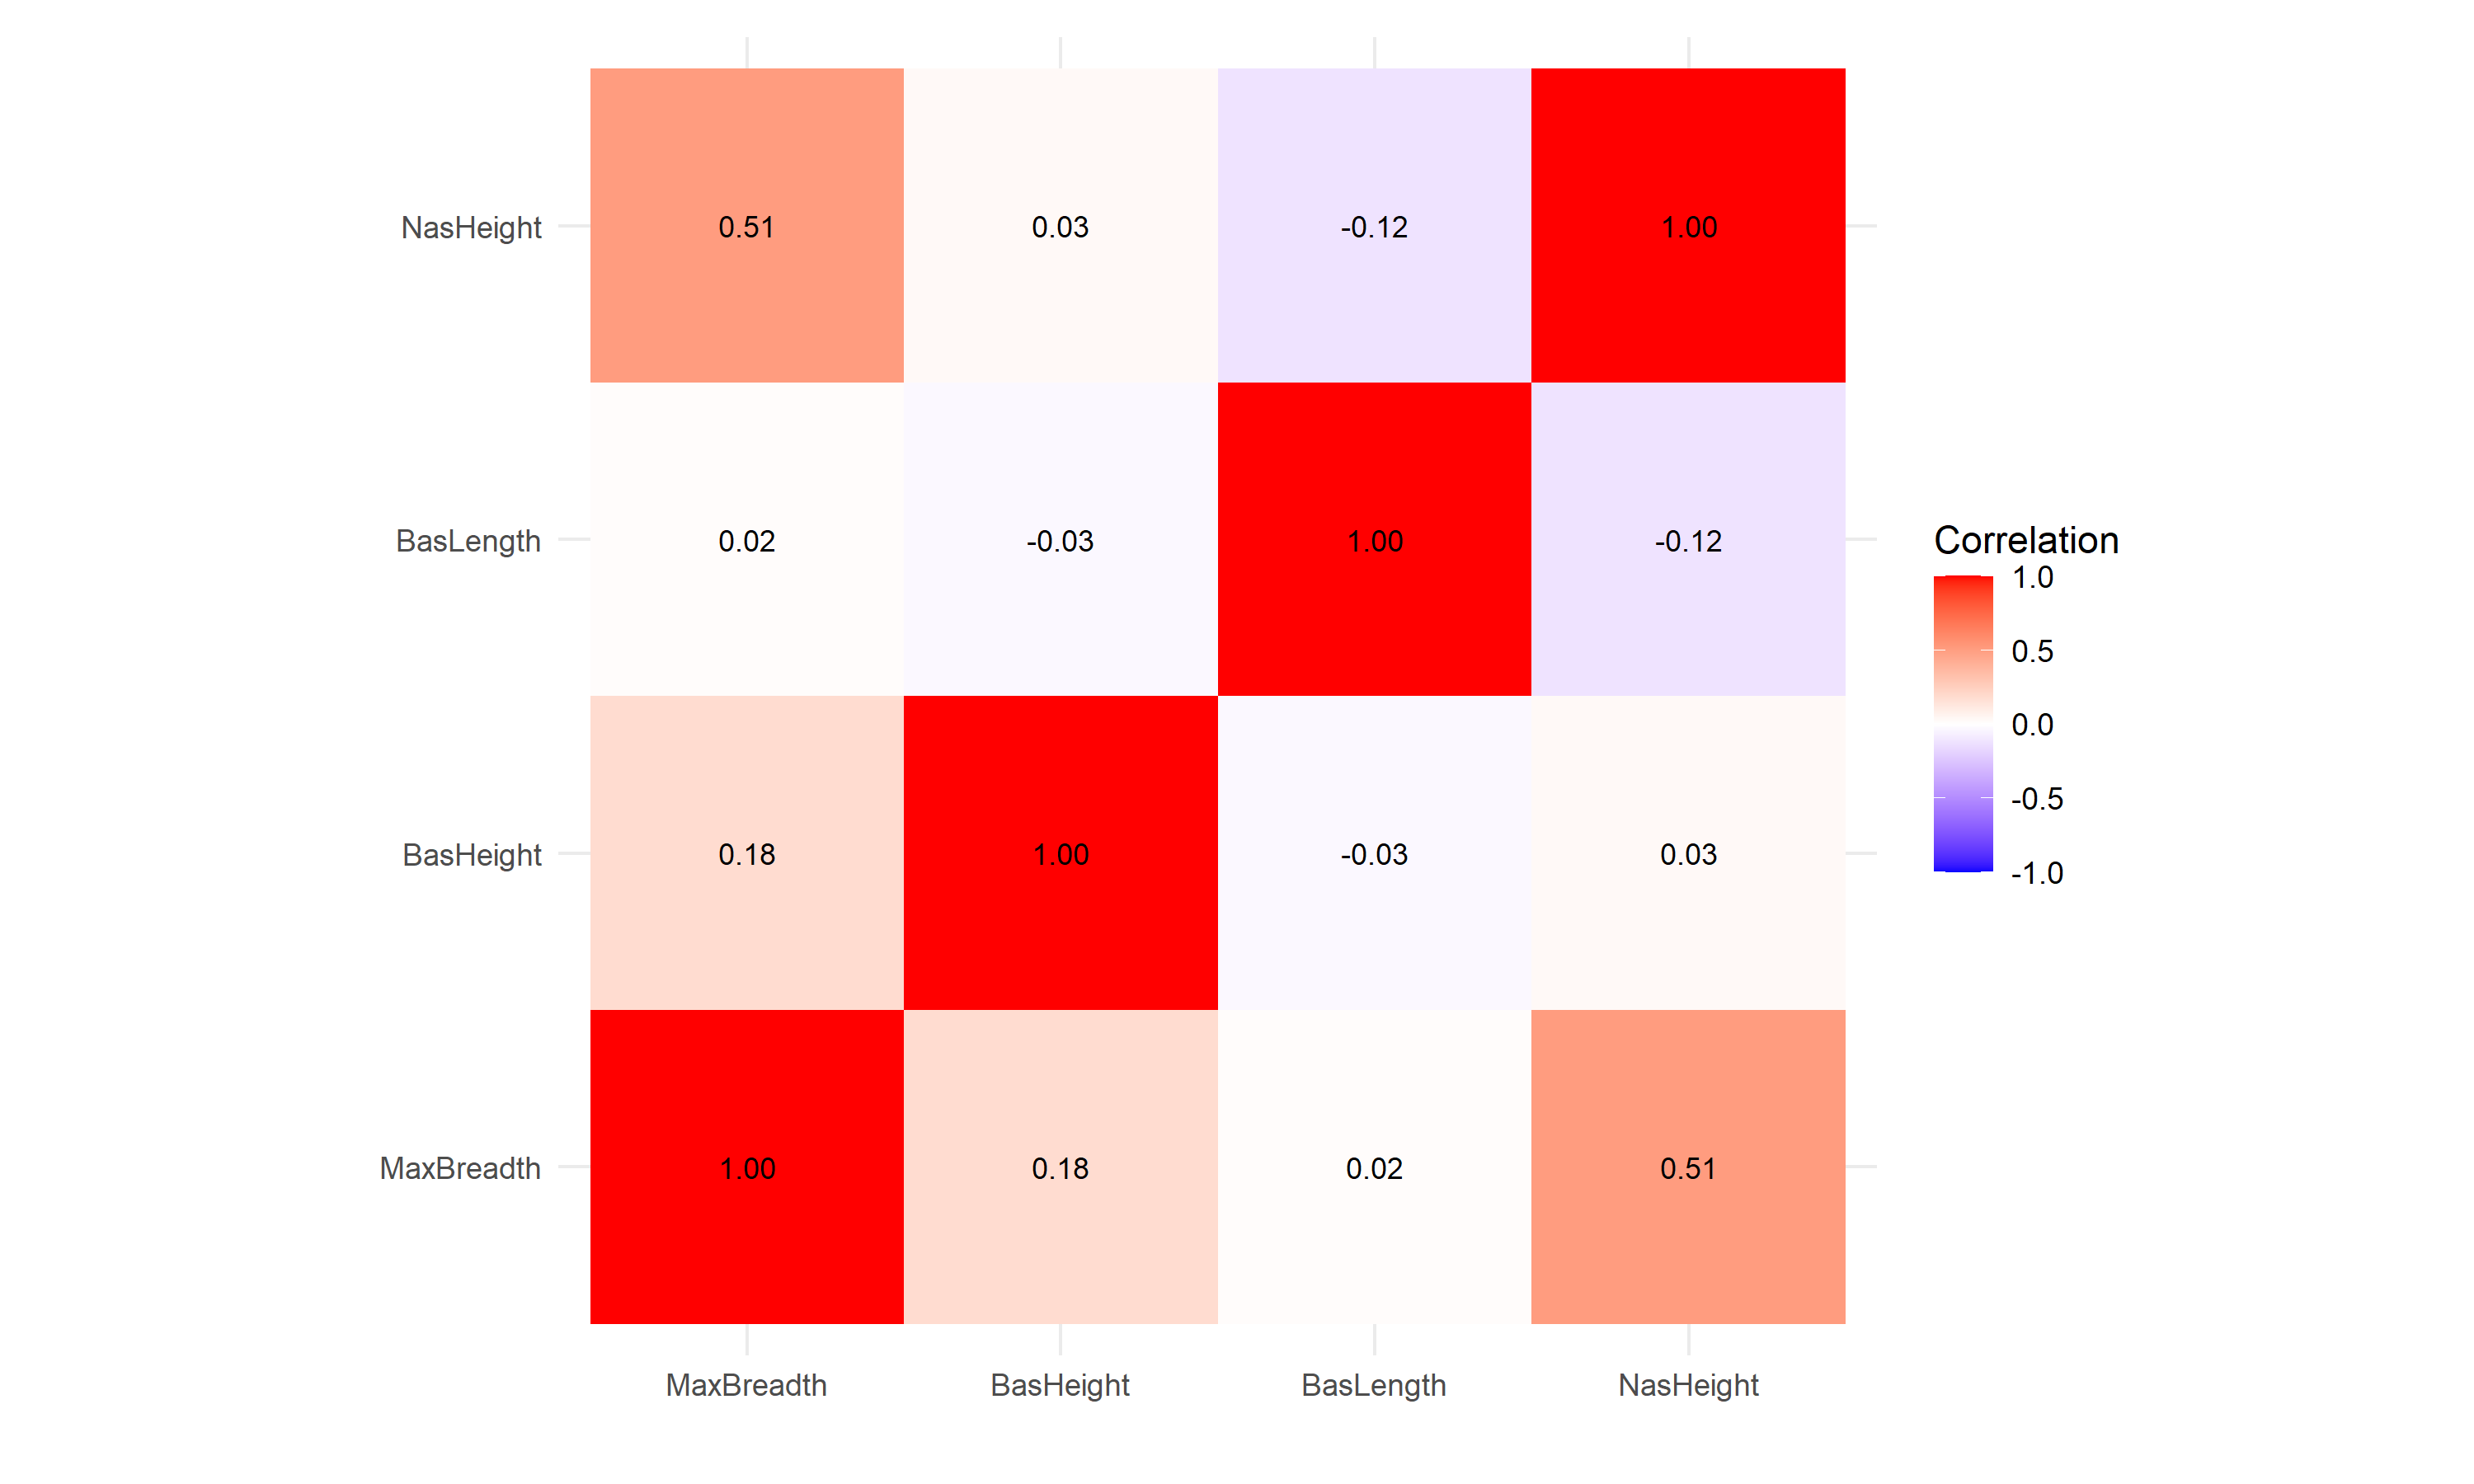
\includegraphics[width=1\textwidth,height=\textheight]{correlation_heatmaps.png}
\newpage

\begin{itemize}
  \item Over the 5 time periods, The correlation between NasHeight and MaxBreath decreases from an initial strongly positive correlation(0.51) to a very weak negative correlation(-0.1).
  \item From time period 1 to time period 5, The correlation between BasLength and BasHeight increases from a very weak negative correlation(-0.03) to a strong positive correlation(0.47)
  \item There is no pattern observed over the time periods between BasHeight and NasHeight
  \item Between time period 1 and time period 4, the correlation between NasHieght and BasLength increases from a weak negative correlation(-0.12) to a strong positive correlation(0.41), however the correlation weakens in Period 5.
  \item From time period 2 to time period 5, the correlation between BasLength and MaxBreath, decreases from a slightly weak positive correlation(0.23) to a weak negative correlation(-0.07)
  \item From time period 1 to time period 4, the correlation between BasHeight and MaxBreath decreases from a weak positive correlation(0.18) to a weak negative correlation(-0.28). And there is almost no correlation in Period 5.
\end{itemize}

\section{Question 3}
\subsection{Deviation Vectors}

The deviation vector defines the deviation of the observed values from
the variable means, as shown below: \[
\underline{d}_{i} = \underline{x} - \bar{x}\underline{1}
\] In this case, we have to find the angle between the deviation vectors
for X1\{\(\underline{d}_{1}\)\} and X3\(\underline{d}_{3}\) in period 1.

We know that to find the angle: \[
cos(\theta) = \frac{\underline{d}_{1}^{T}\underline{d}_{3}}{||\underline{d}_{1}||.||\underline{d}_{3}||}
\] The distance is calculated as: \[
||\underline{d}_{i}|| =  \sqrt{\underline{d}_{i}^{T}\underline{d}_{i}}
\] The distance for deviation vector 1(\{\(\underline{d}_{1}\)\}) is
27.622, while The distance for deviation vector
3(\{\(\underline{d}_{3}\)\}) is 31.689.

Therefore with this information we find that the \(cos(\theta)\) value
is equal to 0.0150425.

The cosine of the angle between two deviation vectors is equal to the
correlation coefficient between the corresponding vectors: \[
cos(\theta) = \frac{s_{13}}{\sqrt{s_{11}}.\sqrt{s_{33}}}
\] From the information above, the angle between the two deviation
vectors is calculated as: 1.555753 radians or 89.1381 degrees.

We define the following deviation vectors for period 1 across the first
two observations \begin{align}
\begin{bmatrix} 
  3 & -3  \\
  3.5 & -3.5 \\
  -1.5 & 1.5 \\
  0.5 & -0.5
\end{bmatrix}
\end{align}

\section{Question 4}
\subsection{Sample Mean and Covariance}

Researchers are interested in the quantity \(Y_{i} = 3X_{4} − X_{1}\)
for time periods i = 1, . . . , 5.

To calculate the sample mean using the information above, we use the
below formula: \[
E(b^{T}X) = b^{T}\mu
\] We therefore define the appropriate b vector to be: \begin{align}
\mathbf{b} = \begin{bmatrix} -1\\0\\0\\3 \end{bmatrix}
\end{align}

Therefore using the vector above with the mean matrix from question 1,
we have the that sample mean is calculated as below: \begin{align}
\mathbf{E(b^{T}X)} = \begin{bmatrix} 20.233\\18.333\\17.233\\20.400\\17.9333 \end{bmatrix}
\end{align}

There covariance matrix of
\(Y = [Y_{1}\quad Y_{2}\quad Y_{3}\quad Y_{4}\quad Y_{5}]^{T}\) is given
below: \begin{align}
\begin{bmatrix} 
  51.564 & 1.402 & 23.323 & -7.924  & 0.223 \\
  1.402 & 90.712 & -6.080 & 29.862 & 2.885 \\
  23.323 & -6.080460 & 120.11609 & -10.131034 & -33.4321839 \\
  -7.924 & 29.862 & -10.131 & 74.731  & 14.648 \\
   0.223 & 2.885 & -33.432  & 14.648 & 165.029
\end{bmatrix}
\end{align}

\newpage
\section{Appendix}

\begin{Shaded}
\begin{Highlighting}[]
\NormalTok{knitr}\SpecialCharTok{::}\NormalTok{opts\_chunk}\SpecialCharTok{$}\FunctionTok{set}\NormalTok{(}\AttributeTok{warning=}\ConstantTok{FALSE}\NormalTok{,}
                      \AttributeTok{message =} \ConstantTok{FALSE}\NormalTok{,}
                      \AttributeTok{echo =} \ConstantTok{TRUE}\NormalTok{,}
                      \AttributeTok{fig.width =} \DecValTok{5}\NormalTok{,}
                      \AttributeTok{fig.height =} \DecValTok{5}\NormalTok{,}
                      \AttributeTok{fig.align =} \StringTok{"center"}\NormalTok{)}
\FunctionTok{rm}\NormalTok{(}\AttributeTok{list =} \FunctionTok{ls}\NormalTok{())}
\CommentTok{\#setwd("C:/Users/mjmaf/OneDrive/Documents/Hons Multivariate 2024/Assessment1")}

\CommentTok{\# Load the necessary library}
\FunctionTok{library}\NormalTok{(dplyr)}
\FunctionTok{library}\NormalTok{(reshape2)}
\FunctionTok{library}\NormalTok{(ggplot2)}
\FunctionTok{library}\NormalTok{(patchwork)}
\FunctionTok{library}\NormalTok{(tidyr)}

\CommentTok{\# Read the dataset}
\NormalTok{data }\OtherTok{\textless{}{-}} \FunctionTok{read.csv}\NormalTok{(}\StringTok{"CA1.csv"}\NormalTok{, }\AttributeTok{header =} \ConstantTok{TRUE}\NormalTok{)}
\FunctionTok{str}\NormalTok{(data)}
\CommentTok{\#Question 1}
\CommentTok{\# Compute the sample mean vectors for each time period}
\NormalTok{mean\_vectors }\OtherTok{\textless{}{-}}\NormalTok{ data }\SpecialCharTok{\%\textgreater{}\%}
  \FunctionTok{group\_by}\NormalTok{(TimePeriod) }\SpecialCharTok{\%\textgreater{}\%}
  \FunctionTok{summarise}\NormalTok{(}
    \AttributeTok{MaxBreadth =} \FunctionTok{mean}\NormalTok{(MaxBreadth, }\AttributeTok{na.rm =} \ConstantTok{TRUE}\NormalTok{),}
    \AttributeTok{BasHeight =} \FunctionTok{mean}\NormalTok{(BasHeight, }\AttributeTok{na.rm =} \ConstantTok{TRUE}\NormalTok{),}
    \AttributeTok{BasLength =} \FunctionTok{mean}\NormalTok{(BasLength, }\AttributeTok{na.rm =} \ConstantTok{TRUE}\NormalTok{),}
    \AttributeTok{NasHeight =} \FunctionTok{mean}\NormalTok{(NasHeight, }\AttributeTok{na.rm =} \ConstantTok{TRUE}\NormalTok{)}
\NormalTok{  )}

\NormalTok{mean\_vectors}
\CommentTok{\#Qtn 2 function}
\CommentTok{\# Function to generate a heat map for a given time period}
\NormalTok{generate\_heat\_map }\OtherTok{\textless{}{-}} \ControlFlowTok{function}\NormalTok{(time\_period) \{}
\NormalTok{  filtered\_data }\OtherTok{\textless{}{-}}\NormalTok{ data[data}\SpecialCharTok{$}\NormalTok{TimePeriod }\SpecialCharTok{==}\NormalTok{ time\_period,]}
\NormalTok{  cor\_matrix }\OtherTok{\textless{}{-}} \FunctionTok{cor}\NormalTok{(filtered\_data[,}\DecValTok{1}\SpecialCharTok{:}\DecValTok{4}\NormalTok{]) }\CommentTok{\# Assuming the first four columns are the variables}

  \CommentTok{\# Melt the correlation matrix for ggplot}
\NormalTok{  melted\_cor\_matrix }\OtherTok{\textless{}{-}} \FunctionTok{melt}\NormalTok{(cor\_matrix)}

  \CommentTok{\# Plot}
  \FunctionTok{ggplot}\NormalTok{(melted\_cor\_matrix, }\FunctionTok{aes}\NormalTok{(}\AttributeTok{x =}\NormalTok{ Var1, }\AttributeTok{y =}\NormalTok{ Var2, }\AttributeTok{fill =}\NormalTok{ value)) }\SpecialCharTok{+}
    \FunctionTok{geom\_tile}\NormalTok{() }\SpecialCharTok{+}
    \FunctionTok{geom\_text}\NormalTok{(}\FunctionTok{aes}\NormalTok{(}\AttributeTok{label =} \FunctionTok{sprintf}\NormalTok{(}\StringTok{"\%.2f"}\NormalTok{, value)), }\AttributeTok{color =} \StringTok{"black"}\NormalTok{, }\AttributeTok{size =} \DecValTok{3}\NormalTok{) }\SpecialCharTok{+}
    \FunctionTok{scale\_fill\_gradient2}\NormalTok{(}\AttributeTok{low =} \StringTok{"blue"}\NormalTok{, }\AttributeTok{high =} \StringTok{"red"}\NormalTok{, }\AttributeTok{mid =} \StringTok{"white"}\NormalTok{, }
                         \AttributeTok{midpoint =} \DecValTok{0}\NormalTok{, }\AttributeTok{limit =} \FunctionTok{c}\NormalTok{(}\SpecialCharTok{{-}}\DecValTok{1}\NormalTok{,}\DecValTok{1}\NormalTok{), }\AttributeTok{space =} \StringTok{"Lab"}\NormalTok{, }
                         \AttributeTok{name=}\StringTok{"Pearson}\SpecialCharTok{\textbackslash{}n}\StringTok{Correlation"}\NormalTok{) }\SpecialCharTok{+}
    \FunctionTok{theme\_minimal}\NormalTok{() }\SpecialCharTok{+}
    \FunctionTok{theme}\NormalTok{(}\AttributeTok{axis.text.x =} \FunctionTok{element\_text}\NormalTok{(}\AttributeTok{angle =} \DecValTok{45}\NormalTok{, }\AttributeTok{vjust =} \DecValTok{1}\NormalTok{, }\AttributeTok{size =} \DecValTok{9}\NormalTok{, }\AttributeTok{hjust =} \DecValTok{1}\NormalTok{),}
          \AttributeTok{axis.text.y =} \FunctionTok{element\_text}\NormalTok{(}\AttributeTok{size =} \DecValTok{9}\NormalTok{),}
          \AttributeTok{plot.title =} \FunctionTok{element\_text}\NormalTok{((}\AttributeTok{size =} \DecValTok{14}\NormalTok{))) }\SpecialCharTok{+}
    \FunctionTok{labs}\NormalTok{(}\AttributeTok{x =} \StringTok{\textquotesingle{}\textquotesingle{}}\NormalTok{, }\AttributeTok{y =} \StringTok{\textquotesingle{}\textquotesingle{}}\NormalTok{, }\AttributeTok{title =} \FunctionTok{paste}\NormalTok{(}\StringTok{"Correlation Matrix Heat Map }\SpecialCharTok{\textbackslash{}n}\StringTok{ for Time Period"}\NormalTok{, time\_period))}
\NormalTok{\}}

\CommentTok{\#Q2 cntd}
\CommentTok{\# Generate heat map for time periods}
\NormalTok{time\_periods }\OtherTok{\textless{}{-}} \FunctionTok{unique}\NormalTok{(data}\SpecialCharTok{$}\NormalTok{TimePeriod)}
\NormalTok{plot\_list }\OtherTok{\textless{}{-}} \FunctionTok{list}\NormalTok{()}

\ControlFlowTok{for}\NormalTok{ (time\_period }\ControlFlowTok{in}\NormalTok{ time\_periods) \{}
\NormalTok{  plot\_list[[time\_period]] }\OtherTok{\textless{}{-}} \FunctionTok{generate\_heat\_map}\NormalTok{(time\_period)}
\NormalTok{\}}

\CommentTok{\# Combine the plots. Adjust the layout with \textasciigrave{}plot\_layout()\textasciigrave{}}
\NormalTok{combined\_plot }\OtherTok{\textless{}{-}} \FunctionTok{wrap\_plots}\NormalTok{(plot\_list, }\AttributeTok{ncol =} \DecValTok{3}\NormalTok{) }\SpecialCharTok{+} 
  \FunctionTok{plot\_layout}\NormalTok{(}\AttributeTok{guides =} \StringTok{\textquotesingle{}collect\textquotesingle{}}\NormalTok{)}

\CommentTok{\#save plots}
\FunctionTok{ggsave}\NormalTok{(}\StringTok{"correlation\_heatmaps.png"}\NormalTok{, }\AttributeTok{plot =}\NormalTok{ combined\_plot, }\AttributeTok{width =} \DecValTok{10}\NormalTok{, }\AttributeTok{height =} \DecValTok{6}\NormalTok{, }\AttributeTok{units =} \StringTok{"in"}\NormalTok{)}
\CommentTok{\# Q3}

\CommentTok{\# Filter data for period 1}
\NormalTok{data\_period\_1 }\OtherTok{\textless{}{-}}\NormalTok{ data[data}\SpecialCharTok{$}\NormalTok{TimePeriod }\SpecialCharTok{==} \DecValTok{1}\NormalTok{,]}

\CommentTok{\# Extract vectors for X1 and X3}
\NormalTok{x1 }\OtherTok{\textless{}{-}}\NormalTok{ data\_period\_1}\SpecialCharTok{$}\NormalTok{MaxBreadth}
\NormalTok{x3 }\OtherTok{\textless{}{-}}\NormalTok{ data\_period\_1}\SpecialCharTok{$}\NormalTok{BasLength}

\CommentTok{\# Compute deviation vectors from their means}
\NormalTok{x1\_dev }\OtherTok{\textless{}{-}}\NormalTok{ x1 }\SpecialCharTok{{-}} \FunctionTok{mean}\NormalTok{(x1)}
\NormalTok{x3\_dev }\OtherTok{\textless{}{-}}\NormalTok{ x3 }\SpecialCharTok{{-}} \FunctionTok{mean}\NormalTok{(x3)}

\CommentTok{\# Calculate the cosine of the angle using the dot product}
\NormalTok{cos\_angle }\OtherTok{\textless{}{-}} \FunctionTok{sum}\NormalTok{(x1\_dev }\SpecialCharTok{*}\NormalTok{ x3\_dev) }\SpecialCharTok{/}\NormalTok{ (}\FunctionTok{sqrt}\NormalTok{(}\FunctionTok{sum}\NormalTok{(x1\_dev}\SpecialCharTok{\^{}}\DecValTok{2}\NormalTok{)) }\SpecialCharTok{*} \FunctionTok{sqrt}\NormalTok{(}\FunctionTok{sum}\NormalTok{(x3\_dev}\SpecialCharTok{\^{}}\DecValTok{2}\NormalTok{)))}
\NormalTok{cos\_angle}
\CommentTok{\# Calculate the angle in radians}
\NormalTok{angle\_radians }\OtherTok{\textless{}{-}} \FunctionTok{acos}\NormalTok{(cos\_angle)}

\CommentTok{\# Convert the angle to degrees}
\NormalTok{angle\_degrees }\OtherTok{\textless{}{-}}\NormalTok{ angle\_radians }\SpecialCharTok{*}\NormalTok{ (}\DecValTok{180} \SpecialCharTok{/}\NormalTok{ pi)}

\NormalTok{angle\_degrees}
\CommentTok{\#Qtn 4}
\NormalTok{b }\OtherTok{\textless{}{-}} \FunctionTok{c}\NormalTok{(}\SpecialCharTok{{-}}\DecValTok{1}\NormalTok{,}\DecValTok{0}\NormalTok{,}\DecValTok{0}\NormalTok{,}\DecValTok{3}\NormalTok{)}
\NormalTok{means\_matrix }\OtherTok{\textless{}{-}} \FunctionTok{as.matrix}\NormalTok{(mean\_vectors[, }\DecValTok{2}\SpecialCharTok{:}\FunctionTok{ncol}\NormalTok{(mean\_vectors)])}
\NormalTok{y\_means }\OtherTok{\textless{}{-}}\NormalTok{ means\_matrix}\SpecialCharTok{\%*\%}\NormalTok{b}
\CommentTok{\#means for y1 to y5}
\NormalTok{y\_means}

\CommentTok{\#now calculating the covariance matrix}
\NormalTok{data }\OtherTok{=}\NormalTok{ data }\SpecialCharTok{\%\textgreater{}\%} \FunctionTok{mutate}\NormalTok{(}\AttributeTok{Y =} \DecValTok{3}\SpecialCharTok{*}\NormalTok{NasHeight }\SpecialCharTok{{-}}\NormalTok{ MaxBreadth) }\CommentTok{\#the y value for each data data point}
\NormalTok{y\_data }\OtherTok{\textless{}{-}}\NormalTok{ data }\SpecialCharTok{\%\textgreater{}\%} \FunctionTok{select}\NormalTok{(TimePeriod, Y)}

\CommentTok{\#create an index to match data points ie 30 data points for 5 periods}
\NormalTok{index }\OtherTok{\textless{}{-}} \FunctionTok{rep}\NormalTok{(}\FunctionTok{seq}\NormalTok{(}\DecValTok{1}\NormalTok{,}\DecValTok{30}\NormalTok{), }\AttributeTok{times =} \DecValTok{5}\NormalTok{)}
\NormalTok{y\_data}\SpecialCharTok{$}\NormalTok{index }\OtherTok{\textless{}{-}}\NormalTok{ index}
\NormalTok{y\_data\_wide }\OtherTok{\textless{}{-}} \FunctionTok{pivot\_wider}\NormalTok{(y\_data, }\AttributeTok{names\_from =}\NormalTok{ TimePeriod, }\AttributeTok{values\_from =}\NormalTok{ Y) }\CommentTok{\#pivot data to use cov function}

\FunctionTok{head}\NormalTok{(y\_data\_wide)}
\NormalTok{y\_data\_wide }\OtherTok{\textless{}{-}}\NormalTok{ y\_data\_wide }\SpecialCharTok{\%\textgreater{}\%} \FunctionTok{select}\NormalTok{(}\SpecialCharTok{{-}}\NormalTok{index) }\CommentTok{\#remove the index from cov calculation}
\NormalTok{y\_covariances }\OtherTok{\textless{}{-}} \FunctionTok{cov}\NormalTok{(y\_data\_wide)}
\NormalTok{y\_covariances}
\end{Highlighting}
\end{Shaded}


\end{document}
